\documentclass{kit}

\author{Julius Vater - 2603322}
\title{Betriebssysteme}
\begin{document}
\maketitle
\tableofcontents
\pagebreak
\section{OS - Tasks and Responibilities}
  \begin{itemize}
    \item Abstraction / Standartisisation
    \item Resource menagement
    \item Security and Protection
    \item Provide an execution environment for applications
  \end{itemize}
  \subsection{Three Easy Pieces}
    \begin{itemize}
      \item Virtualization
      \item Concurrency
      \item Persistence
    \end{itemize}
\section{\textbf{A}pplication \textbf{B}inary \textbf{I}nterface (ABI)}
  Specifies
  \begin{itemize}
    \item Interface of binary programms
    \item Instruction set
    \item Calling convention
    \item Basic data types and ther size / alignment
    \item How to perform System Calls
  \end{itemize}
\section{Multiprogramming}
  Allows multiple processes to run concurrently. There are two possible broad categories to share a CPU:
  \subsection{Cooperative Multitasking}
    \begin{itemize}
      \item Process \textbf{voluntarily} yield control so another on can take over\\
        (Typically when they are blocking on some I/O of have finished their job for now
      \item Problems / Advanteges:
        \begin{itemize}
          \item A bad actor or buggy program can bring the whole system to its knee 
          \item It can lead to easier programs, as you can just assume you are never interrputed
        \end{itemize}
    \end{itemize}
    \subsection{Preemption}
      \begin{itemize}
        \item Processes get periodically interrupted by \textbf{Timer-interrupts}
        \item This transfers control to the OS, which can choose to schdulte another process instead
      \end{itemize}
    \subsection{CPU / I/O-bound Proscesses}
      \begin{itemize}
        \item CPU-bound: Process that rarely invokes I/O, unlikely to block
        \item I/O-bound: Often blocks to wait for I/O, perfomrs short CPU-bursts in between
      \end{itemize}

%---------------------------------------------------------------------------------------------------------------------------

\section{C-Basics}
  \subsection{Datatypes}
    \begin{tabular}{ccc}
      Name & Minmal size in Bytes & Size for me in Bytes \\ \hline \hline
      char & 1 & 1 \\
      short & 2 & 2 \\
      int & 2 & 4 \\
      float &  & 4 \\
      double &  & 8 \\ \hline
      long & 4 & 8 \\
      long long & 8 & 8 \\ \hline
    \end{tabular}\\\\
    Boolean gibt es nicht. 0 ist false, alles andere ist true.
  \subsection{Arrays}
    \begin{itemize}
      \item Ein zusammenhängeder Speicherbereich
      \item Größe ist Teil eines Typs
    \end{itemize}
  \subsection{Strings}
    \begin{itemize}
      \item Ein char-Array mit Null-Terminator $\Rightarrow$ Ein Byte länger
      \item Nutzen den ASCII code
    \end{itemize}
  \subsection{Structs}
    \begin{itemize}
      \item Komplexerer Datentypen
      \item Zusammengesetzt aus andern Datentypen
      \item \textbf{Keine Klasse} da keine Vererbung oder Methoden
    \end{itemize}
  \subsection{Forward declarations}
    \begin{itemize}
      \item Funktionen müssen vor dem Aufruf deklariert sein
      \item Implementierung kann auch irgendwann später erfolgen
      \item Implementierung zu Entwicklung nicht notwenidig
    \end{itemize}
  \subsection{Header files}
    \begin{itemize}
      \item Aufsplitten in Deklaration und Definition
      \item Nutzer bindet Header zum Programmieren ein, lnkt dann gegen eine Implementierung
    \end{itemize}
  \subsection{Makros}
    \begin{itemize}
      \item Macros in C define constants or inline code eith the \#define direcive
      \item They are processed, meaning they are expanded before actual compilation
      \item commonly used to replace values or create code nippets for repetitve tasks
      \item Macros offer:
        \begin{itemize}
          \item Faster execution by inlining code, avoiding funktion call overhead
          \item Code generation flexibility, such as for debugging or generic functions
        \end{itemize}
    \end{itemize}

%---------------------------------------------------------------------------------------------------------------------------

\section{Fork}
  \begin{itemize}
    \item Creates a mostly identical child process
    \item \begin{itemize}
        \item Same address space layout
        \item Same data (as if was all copied over)
        \item Share open file descriptors
        \item But the child has its own PID and address space
    \end{itemize}
  \end{itemize}
  \newpage
\section{Interrupts}
  \subsection{Three events to invoce the kernel}
    \begin{itemize}
      \item Interrupts
        \begin{itemize}
          \item A signal gernerated outside the processor (typically from an I/O device)
        \end{itemize}
      \item Exceptions
        \begin{itemize}
          \item Caused by the CPU
          \item Inform the operating system of an error condition during execution
        \end{itemize}
      \item Syscalls
        \begin{itemize}
          \item Explicit call from user application into OS
          \item Used to interact with the OS
        \end{itemize}
    \end{itemize}
    \begin{tabular}{c|cc}
       & Voluntarily & Invluntarily \\ \hline
      Sync & System call & Exception \\
      Async & ??? & Interrupt
    \end{tabular}
  \subsection{Trap instruction}
  \begin{enumerate}[label=\arabic*.]
      \item trap is executed and switches the CPU to kernel mode
      \item The CPU continues exection at hardware dependent location
    \end{enumerate}
    $\Rightarrow$ trap can be seen as a low-level instruction making a higher-level mechanism (syscalls) possible
\section{Syscalls}
  The user-level application can't just call a kernel funktion\\
  $\Rightarrow$ The kernel somehow needs to dispatch to the correct funktion
  $\Rightarrow$ Array of funkction pointers with system call numbers as indices
\section{Scheduling basics}
  A Schedular maps processes to resources. Ideally every process gets what it needs some day.\\
  Types of Schedulars:
  \begin{itemize}
    \item CPU-Scheduler    
    \item Disk-Schedular
    \item Network I/O
  \end{itemize}
  \subsection{Long- and Short-Term Schedular}
    \begin{itemize}
      \item LTS: Decide which process to put in the run queue
      \item STS: Decide which process runs on the CPU
    \end{itemize}
    $\Rightarrow$ Reduce degree of multiporgramming, make room in memory\\\\
    Some metrics:
    \begin{itemize}
      \item Processor utilization: Percentage of working time
      \item Throughput: How many jobs do you finish?
      \item Turnaround time: Wallclock-time from submission to finish
      \item Waiting time: How long did it spend in the ready queue
      \item Response time: Time submission of a request and first response (e.g. key press to echo on screen) 
    \end{itemize}
  \subsection{Shortest Job First}
    \begin{itemize}
      \item You would need to have future knowlege to figure otu the job length
      \item Predict the future based on past behaviour
    \end{itemize}
  \subsection{Priorities}
    \begin{itemize}
      \item Each process is assigned a priority
      \item The process with the highest priority is chosen
    \end{itemize}
  \subsubsection{Multi-Level Feedback Queue}
    \begin{itemize}
      \item All processes start in the highest queue
      \item When the use up their timeslice and are preempted, they descend
      \item If the block before, they stay in the level (optionally: Are moved up)
    \end{itemize}
    $\Rightarrow$ I/O bound processes rise to the top and react quickly, CPU bound processes get longer timeslices but less
    often
\section{Process Switching (PCB)}
  When switching processes the kernel needs to adjust:
  \begin{itemize}
    \item Instruction, Base and Frame Pointer
    \item General purpose register
    \item Address space
    \item And a bit of housekeeping: Open files, scheduling priorities, ...
  \end{itemize}
  $\Rightarrow$ These things make up the PCB - The Process Control Block
  \subsection{Process swithing as text}
    \begin{enumerate}[label=\arabic*.]
      \item Transition to the kernel (through Interrupt, Exception, Syscall)
      \item Save the context of the process (Registers, Program counter, Stack pointer, etc.
      \item Where do you save it to? A per-process kernel stack typically (as it is often moved there automatically) and 
        then move it to the PCB
      \item Restore the context of the next process
      \item Leave kernel mode and transfer controll to the PC of the next process
    \end{enumerate}
\section{Threads}
  \begin{itemize}
    \item A thread is an entity of execution, the personification of control flow
    \item A thread lives in an address space, i.e. all the addresses that it can access and the data are stored there
    \item Thread + Address Space = Process
  \end{itemize}
  \subsection{Thread models}
    \begin{itemize}
      \item Many To One: The kernel only knows one of possibly multiple thready multiple threads
      \item One To One: Each user thread maps to a kerne thread
      \item M To N: Flexible mapping of user threads to kernel threads
    \end{itemize}
  \subsection{Kernel Mode Threads - Kernel Level Threads}
    \begin{itemize}
      \item Kernel Level Thread: The kernel knows about and manages the thread
      \item Kernel Mode Thread: The thread runs in kernel mode
    \end{itemize}
    Why do you need kernel mode threads?
    \begin{itemize}
      \item Sometimes the OS needs to do some housekeeping that doesen't belong in a syscall
      \item Free some pages, swap something in and out of memory
      \item Flush pages from disk cache to the hard disk
      \item Perform VFS Checkpointing
      \item ...
    \end{itemize}
\section{Memory Management Basics}
  \subsection{Physical and Virtual Addresses}
    What is the difference
    \begin{itemize}
      \item We assume no 1:1 mapping
      \item All program addresses are virtual
      \item Mapped to physical addresses as needed by the memory management unit (MMU)
    \end{itemize}
  \subsection{Fragmentation}
    \begin{itemize}
      \item Internal: within a block (not the whole block is used
      \item External: due to external factors (free up space, etc.)
    \end{itemize}
    \newpage
  \subsection{Segmentation}
    \begin{multicols}{2}
      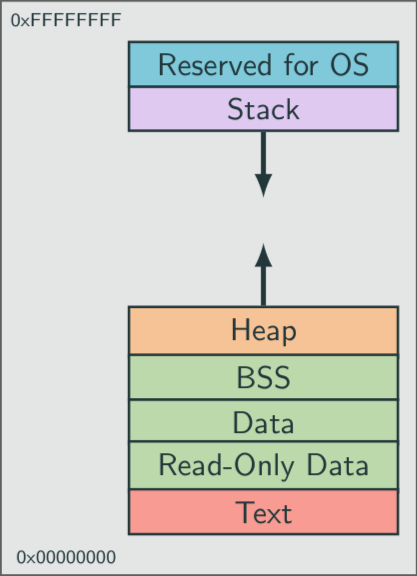
\includegraphics[height=7cm]{img/segmentation.png}\\
      Segmentation means to devide the main memory into mutltiple segments.
    \end{multicols}
  \subsection{Memory allocataion policies}
    \begin{itemize}
      \item First Fit: Pick the first block that ist large enough
      \item Best Fit: Pick the smallest block that fits
      \item Worst Fit: Pick the largest block that fits
    \end{itemize}
    \pagebreak
  \subsection{Allocators}
    \begin{itemize}
      \item Slab allocator:\\\\
        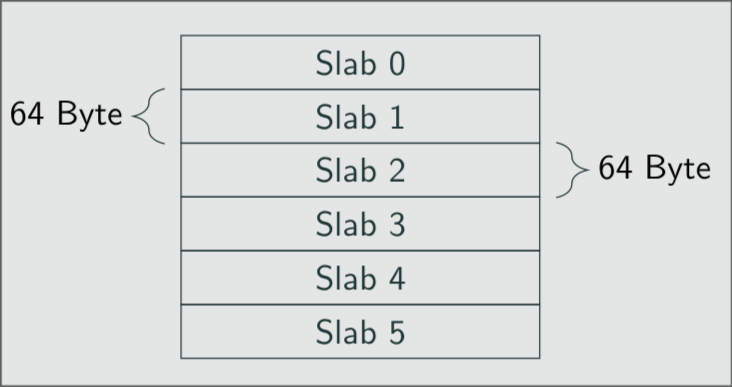
\includegraphics[height=6cm]{img/slab_allocator.png}
      \item Buddy allocator:\\\\
        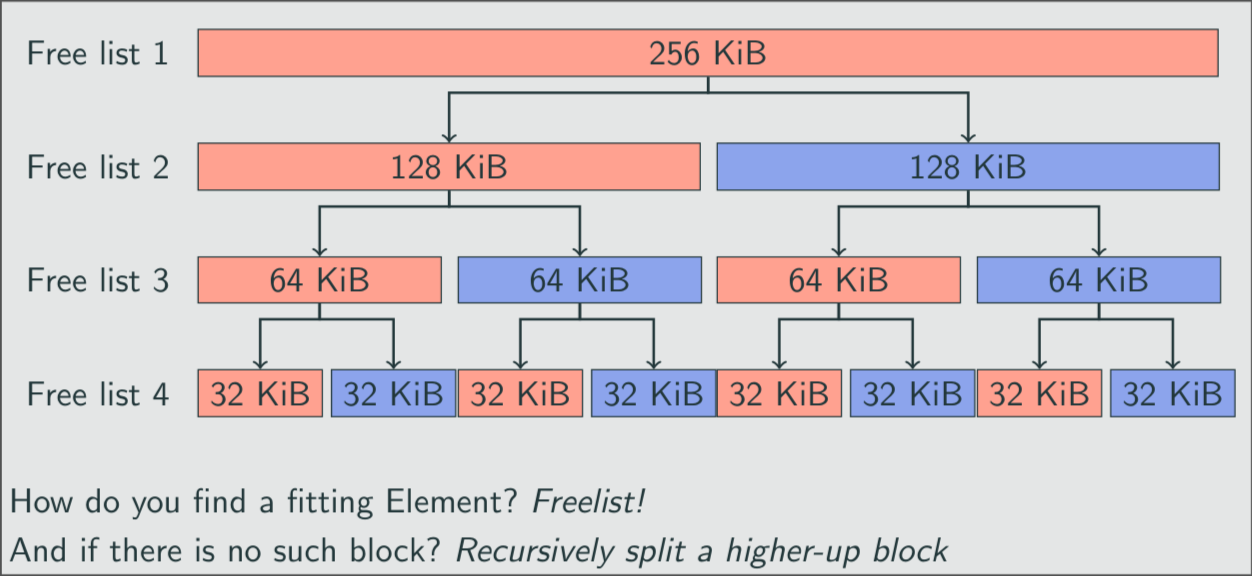
\includegraphics[height=6cm]{img/buddy_allocator.png}
        Internal fragmentation: Power of two blocks (request memory of size $2^k+1$)\\
        External fragmentation: Free every other block in a level
    \end{itemize}
    You can also combine them to allocate large chunkgs with the buddy allocator and small chunkgs within them using the 
    slab allocator.
    \newpage
\section{Paging}
  \begin{itemize}
    \item Virtual memory is broken into fixed-size chunks (pages)
    \item Physical memory is broken into fixed-size chunks of the same size (frame)
    \item Virtual pages are mapped to page frames
    \item Benefits over Segmentation:
      \begin{itemize}
        \item Virtual memory does not need to map to continuous physical memory
        \item Swapping in / out is easier
        \item No external fragmentation, little internal
      \end{itemize}
    \item Segment and Page tables\\\\
      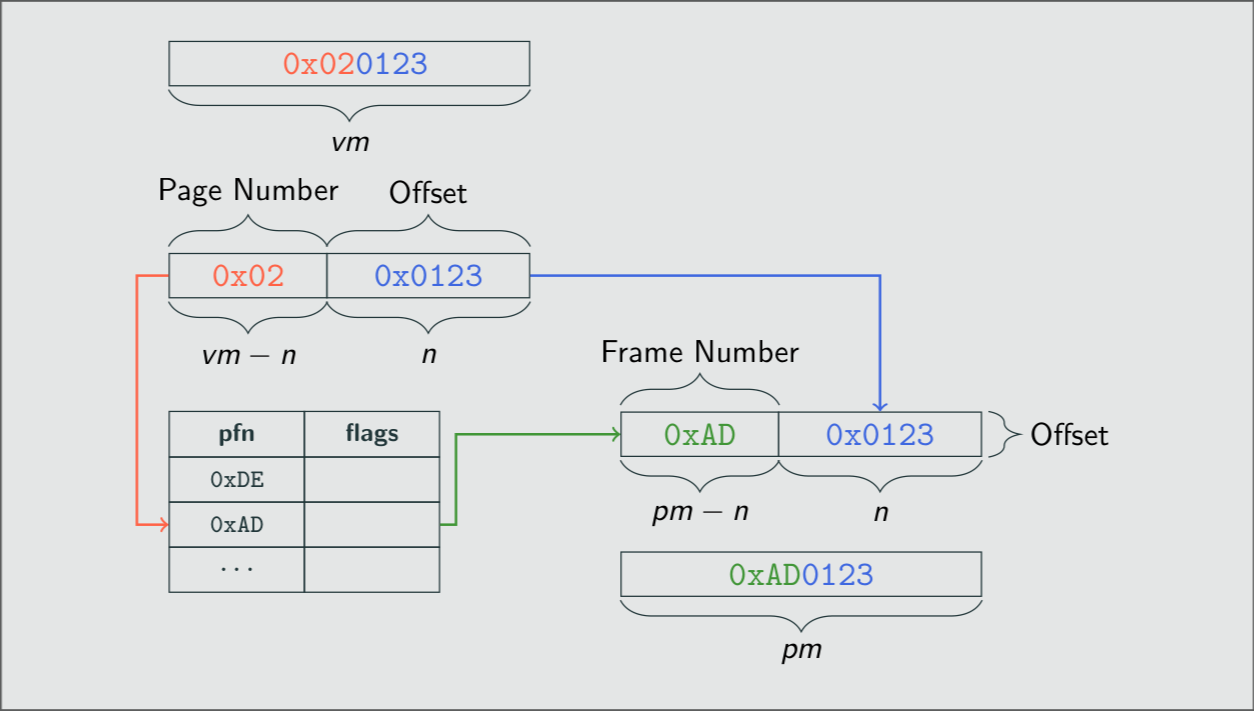
\includegraphics[height=6cm]{img/page_tables.png}
    \item Problems:
      \begin{itemize}
        \item Increases with the size of the size of the virtual address space
        \item 64 Bit AS, 4KiB ($2^{12}$) pages $\Rightarrow n=12\Rightarrow 2^{vm-n}=2^{64-12}=2^{52}$\\
          $\Rightarrow$ If every entry was 1 Bit we'd need 4096 TiB
      \end{itemize}
      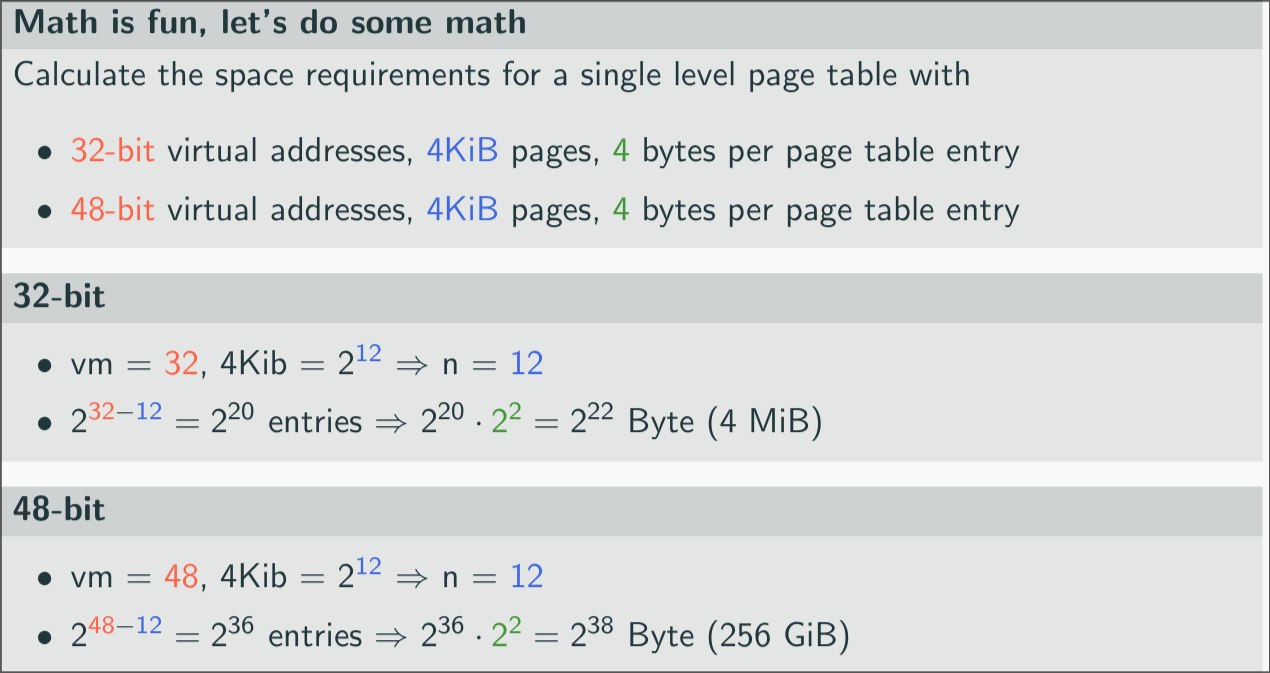
\includegraphics[height=6cm]{img/page_table_math.png}
    \item Multi-Level page tables work the same but with multiple Page Numbers
    \item Inverted Page Tables: Maps physical addresses to virtual ones
    \item Valid/Present Bit: Page might be swapped out, not zeroed yet, ... $\Rightarrow$ Page fualt
  \end{itemize}
  \subsection{Translational Lookaside Buffer (TLB)}
    \begin{itemize}
      \item Lookup from virtual to physical address can be slow
      \item You need to translate addresses all the time\\
        $\Rightarrow$ Can be solved with another caching layer.
      \item TLB caches recently used pages for quick access
      \item TLB-Misses:
        \begin{itemize}
          \item Hardware walked
            \begin{itemize}
              \item Hardware looks at your page table
              \item Hardware resolves the physical address using it
              \item On failure a page fault is raised
              \item Implies, that Page table layout is fixed
            \end{itemize}
          \item Software walked
            \begin{itemize}
              \item Transfers control to TLB miss handler
              \item Kernel routine walks the page table and tries to find a mapping
              \item Loads that mapping into the TLB and can chosse which entry to evict
              \item If there is non $\Rightarrow$ Jump to page fault handler
            \end{itemize}
          \item When is a TLB miss or page fault raised?
            Due to the TLB:
            \begin{itemize}
              \item Software walked: No entry found in TLB $\Rightarrow$ TLB miss exception
              \item Hardware walked: No mapping in page table $\rightarrow$ Page fault
            \end{itemize}
            And other problems: Invalid access to a mapped page
            \begin{itemize}
              \item Software walked: Raise some kind of TLB fault if the page is e.g. read-only
              \item Hardware walked: Page fault raised, page fault handler has to find out what happened
            \end{itemize}
        \end{itemize}
    \end{itemize}
  \subsection{Information stored in the TLB}
    \begin{itemize}
      \item Physical Frame Number, Virtual Page Number
      \item Valid / Present Bit
      \item Modified bit, permissions, ...
    \end{itemize}
  \subsection{Page Faults}
    \begin{itemize}
      \item Demand-Paging: Load pages on-demand, right when they are needed\\
        + Only loads needed data $\Rightarrow$ Less memory wasted\\
        - Generates lots of page faults before working set is in memory
      \item Pre-Paging: Loaded Pages speculatively in batches, even before you need them\\
        + Might reduce number of page faults\\
        + HDDs a lot faster when reading chunks\\
        - Loads more then needed $\Rightarrow$ Wasteful\\
        - More I/O $\Rightarrow$ Slower
      \item Information needed
        \begin{itemize}
          \item Acess flags: Can the user perform the operation on this page?
          \item Where to find the most recent version (differnt for zero filled, file backed, etc.)
        \end{itemize}
    \end{itemize}
  \subsection{Page replacement}
    \begin{itemize}
      \item The pager tries to keep "spare pages"
      \item Replacement algorithms
        \begin{itemize}
          \item Local page replacement algorithms: Only look through the frame of that process
          \item Global page replacement algorithms: Look throug all frames, even that of other processes
        \end{itemize}
      \item Working set: The set of pages that a process accessed in the last $n$ page references
      \item Thrashing: Not enough frames to fit the working set $\Rightarrow$ Pages will be stored to disk and reloaded
        very often
    \end{itemize}
    \subsection{Policies}
      We need to find a victim page to replace with a new one
      \begin{itemize}
        \item FIFO: \textbf{F}irst page to be loadied \textbf{i}n is the \textbf{f}irst to be loaded \textbf{out}
        \item LRU: \textbf{L}east \textbf{r}ecently \textbf{u}sed page is evicted
        \item Optimal: Evict the page that is used the furhtest into the future. (Used as a benschmark)
        \item Clock: Einmal durch alle Einträge gehen und die "Anzahl der Benutzungen" reduzieren, bis ein Eintrag mit 
          null kommt und den ersetzen
      \end{itemize}
\section{Caches}
  \subsection{Types of cache}
    \begin{itemize}
      \item Full Associative: Goes throug the whole cache to find the right entry
      \item Set-Associative: Cache is devided into multiple sets that work "as full assiciative"
      \item Direct Mapped: Every address has a directly mapped entry in the cache
    \end{itemize}
  \subsection{Cache Misses}
    \begin{itemize}
      \item Compulsory Miss: Never accessed that address before
      \item Capacity Miss: Cache was full and it was evicted
    \end{itemize}
  \subsection{Write in Caches}
    What do you do when you write to 
    \begin{itemize}
      \item an address in the cache?
        \begin{itemize}
          \item Write Through: Update the cache and the main memory
          \item Write Back: Update only the cache. Update main memory on eviction
        \end{itemize}
      \item an address not in the cache?
        \begin{itemize}
          \item Write-allocate: First load it into the cache. Then see above
          \item Write-to-memory: Don't laod into cache, modify in memory
        \end{itemize}
    \end{itemize}
  \subsection{Where to place the cache}
      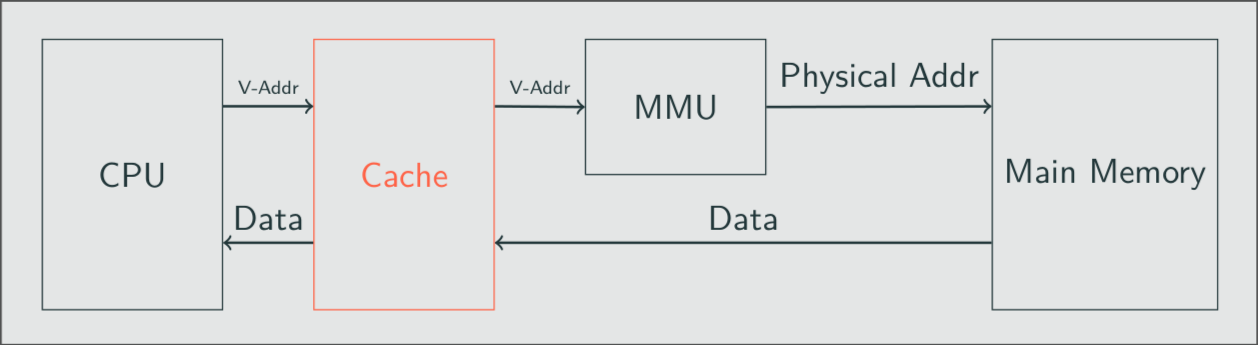
\includegraphics[width=\textwidth]{img/cache_placement_1.png}
      Address: Virtually Index, Virtually Tagged (VIVT)\\
      + Fast, no address translation\\
      - Ambiguity Problem (Same virtual address might point to different physical addresses over time)\\
      - Alias Problem (Multiple virtual addresses might point to the same physical address)\\\\
      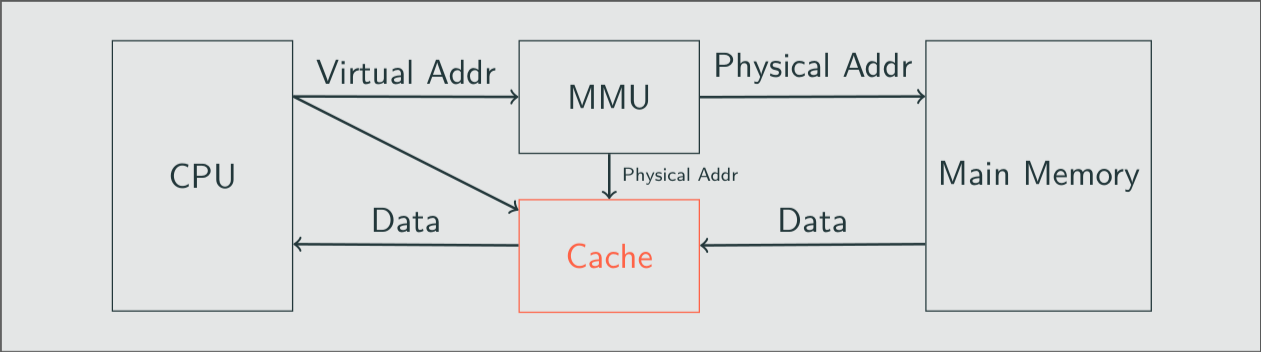
\includegraphics[width=\textwidth]{img/cache_placement_2.png}
      Address: Virtual Indexed, Physically Tagged (VIPT)\\
      + Still relatively fast: Can lookup the index while the MMU works\\
      + Ambiguity solved, as it is tagged by physical address (if entire PFN is uses as a tag)
      - Alias Problem (sometimes)\\\\
      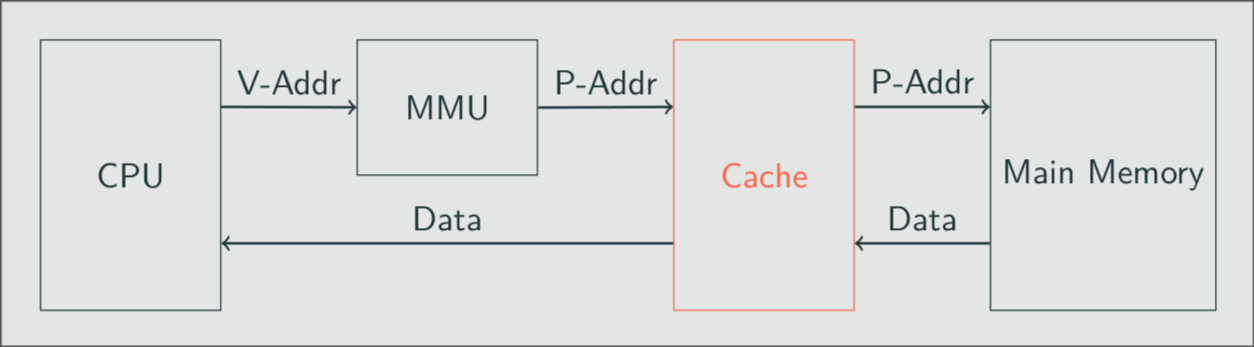
\includegraphics[width=\textwidth]{img/cache_placement_3.png}
      Address: Physically Indexed, Physically Tagged (PIPT)\\
      + Transparent to CPU: no alias, no ambiguity\\
      + Coherency can be implemented in hardware\\
      - Allocation conflicts
      \newpage
\section{Inter-Process-Communication (IPC)}
  Different (concurrent) activities can interact via:
  \begin{itemize}
    \item Shared memory (implicitly as they share an address space and explicitly via a shared memory area)
    \item OS facilities (e.g. messages, pipes, Signals, sockets)
    \item High level abstraction (files, database entries)
  \end{itemize}
  \subsection{IPC Buffering}
    Asynchronous sent but not yet recieved messages need to be buffered somewhere:
    \begin{itemize}
      \item Buffering in the Receivers's Address Space\\
        (Does not scale well. You either allow every sender to allocate memory for you or you might run out with many 
        clients)
      \item Buffering in the Kernel\\
        (Does not scale well. You either allow every sender to allocate kernel memory or you might run out with many 
        clients)
      \item Buffering in the Sender's Address Space\\
        + We only need to store it once: The sender has it in a buffer somewhere anyways\\
        + Scales better, as each sender keeps their messages\\
        $\pm$ We need to tell the client when it can reclaim the buffer
    \end{itemize}
    You can emulate asynchronous IPC using synchronous IPC by using a Proxy thread by
    \begin{enumerate}[label=\arabic*.]
      \item Copiing message to the proxy thread
      \item The Proxy thread synchronously sends and might block until recipient calls receive
    \end{enumerate}
    + Allows async I/O
    - Can only send one message per thread
\section{Race Conditions}
  Race conditions happen, when to two processes try to write to the same variable. It is possible, that process A writes 
  someting to the variable but process B overrides it directely.\\
  \subsection{Critical Sections}
    \begin{itemize}
      \item Mutual Exclusion: Only one thread can enter the critical section at once
      \item Bounded Waiting: There is an upper bound on how many different threads can enter the CS while thread is waiting
      \item Progress: Threads in the remainder section do not prevent threads from entering the critical section
      \item Performance: The time overhead of the synchronization primitve is low
    \end{itemize}
  \subsection{Synchronization Primitives}
    \begin{itemize}
      \item Spinnlock
        \begin{itemize}
          \item lock / unlock
          \item Busy-waiting and atomic instructions (e.g compare-and-set)
            \item Recommended for short critical sections as it wastes CPU time
            \item Preemption wastes more resources (threads can't make progress)
            \item $\Rightarrow$ Mostly used in the kernel without interrupts
        \end{itemize}
      \item Semaphore
        \begin{itemize}
          \item wait(sem) (also called acquire) ) signal(sem) (also called release / post)
          \item Has an internal counter that is decremented (wait) or incremented (signal)
          \item Blocks if you try to devrement it below 0
          \item Can be used to implement bounded buffers
        \end{itemize}
      \item Mutex (Binary Semaphore)
        \begin{itemize}
          \item lock(m), unlock(m)
          \item Or a Semaphore with values 0 and 1
        \end{itemize}
    \end{itemize}
  \subsection{Kernel Synchronization}
    How could you achieve mutual exclusion on Single-Core systems?\\
    Masking interrupts. Only one thread can run at a time disabling interrupts prevents preemtion (and other interrupt
    handlers)\\
    Doesent work on Multi-Core-Systems because masking only affects the current CPU. Another core coulb be in the same
    routines and access the same data 
  \subsection{Mutual Exclusion in the kernel}
    \begin{itemize}
    \item The Big kernel Lock:\\
      Have a big lock for the whole kernel. The kernel effectively serialises access\\
      $\Rightarrow$ Can't make use of your processors if you have many syscalls
    \item Fine Grained Lock:\\
      + Only lock areas that are relevant for the current task ($\Rightarrow$ Have many small locks)\\
      - Complex and error prone
    \item Spinlock and Interrupt handlers:\\r
      Without diabling interrupts there is a problem: Lockhold Preemption
      \begin{enumerate}[label=\arabic*.]
        \item Thread enters spinlock
        \item Thread gets pre-empted by interupt handler
        \item Interput handler needs the same lock $\Rightarrow$ Can never acquire it
      \end{enumerate}
      $\Rightarrow$ You might still need to disable interrupts for those
    \end{itemize}
\section{Deadlocks}
\end{document}
